\section{Pipeline}\label{sec:pipeline}

The pipeline consists of three main components: the \textit{Question Generator}, the \textit{Answer Generator}, and the \textit{QA Refinement Generator}.

\begin{figure}[h]
  \centering
  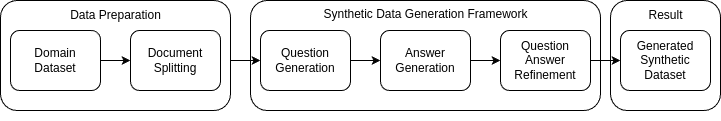
\includegraphics[width=\textwidth]{methodology-overview.png}
  \caption{An overview of our synthetic data generation framework. Given a user-provided domain dataset, our
framework will employ small language models to create a synthetic dataset that can be used
to fine-tune a LLM for downstream Question Answering tasks.}
\end{figure}

\subsection{Data Preparation}
For the source dataset used in our framework, we used ArXiv papers published after 2024, specifically papers relevant to
small language models, fine-tuning LLM's and synthetic data generation.
This choice was motivated by several factors including:
\begin{itemize}
  \item Recent papers ensure that the content was not part of the pre-training data for the LLMs used in our framework
  \item The ease of access to the dataset, which is publicly available and well-structured
  \item Academic papers provide structured factual content that can be used to generate questions and answers and as a proxy for
  domain-specific data in other applications
\end{itemize}

To prepare the data into our framework, we chunked each paper into a fixed size and extracted the title to be used in the
question generator. 

\subsection{Question Generator}\label{sec:question-generator}

In the first step of the pipeline, the Question Generator takes the title of the paper along with a chunk of text from the paper
and generates an initial set of questions that can be answered using the text. To facilitate the generation of diverse questions,
we used a small language model to generate a mix of 'what', 'why', 'how', 'where', and 'summarize' questions, the full prompt can be found in the appendix?.

For each question in our framework, we ensure that the title information is included in the question to serve as context during fine-tuning. We hypothesize
that by including the title in the question, the model will be able to better retrieve the correct answer during downstream zero-shot question answering tasks on the fine-tuned
model. Intuitively, this serves as a form of conditioning for the language model during generation. See section ~\ref{sec:source-results} for more details.

To minimize generating duplicate or similar questions, we leverage a similarity check using the cosine similarity between the embeddings of the generated questions
and remove questions that have high similarity.

\subsection{Answer Generator}

Following the generation of questions, the Answer Generator takes the generated questions and the corresponding text chunk and generates answers for each of the questions.
In this step, we prioritize factual accuracy, organized structure of the response, and clarity. This step can be seen as a simple form of question answering, where the model is
tasked with generating the answer to a question given the context of the text chunk.

\subsection{QA Refinement Generator}
To refine each question-answer pair, we generate a new set of questions that are based on the original question and the answer pair
with the goal of generating questions that approaches the original question from a different angle. This step is critical in
generating more diverse qa pairs while also generating questions that are more challenging and involve more reasoning than the original question.

We generate an answer for each of the refined questions using a similar process as the Answer Generator but using the original answer
and smaller chunks retrieved from a similarity search as context. The extra step in retrieving smaller chunks of text is to ensure that the model
has context to answer the question that is not directly in the original text chunk. Intuitively, we take inspiration from Retrieval Augmented Generation
(RAG) frameworks using vector databases to generate answers in the QA Refinement Generator.

\subsection{Result}

Upon completion of the pipeline, we have a set of question-answer pairs that can be used to fine-tune a small language model for downstream QA tasks.
We perform simple heuristics to ensure that questions that could not be answered or may not exist in the original text are removed from the dataset.

\subsection{Algorithm}

\begin{algorithm}[H]
  \SetAlgoLined
  \KwData{PDF documents $D$, document chunk size $c_d$, retrieval chunk size $c_r$ $(c_d > c_r)$, overlap sizes $(o_d, o_r)$}
  \KwResult{Set of question-answer pairs $QA$}
  
  Initialize vector store $V$ and empty result set $QA$\;
  \ForEach{document $d \in D$}{
      Extract metadata (title, source) from $d$\;
      Chunk document into segments of size $c_d$ with overlap $o_d$\;
      
      \tcp{Embedding Pipeline for RAG}
      Create smaller retrieval chunks of size $c_r$ with overlap $o_r$ from document\;
      Embed retrieval chunks and store embeddings in vector store $V$\;
      
      \tcp{Question Generation Phase}
      \ForEach{document chunk $c$ of size $c_d$}{
          Generate base questions $Q_b$ using LLM\;
          Remove similar questions using embedding similarity\;
          Add source information to questions $Q_b$\;
          \ForEach{question $q \in Q_b$}{
              Generate answer $a$ using document chunk $c$ as context\;
              Add $(q,a)$ to base QA pairs\;
          }
      }
      
      \tcp{Question Refinement Phase}
      \ForEach{$(q,a)$ in base QA pairs}{
          Generate refined questions $Q_r$ based on $(q,a)$\;
          Remove similar questions using embedding similarity\;
          Add source information to questions $Q_r$\;
          \ForEach{question $q_r \in Q_r$}{
              Retrieve top $k$ most similar retrieval chunks $c_r$ from $V$\;
              Generate refined answer using retrieved chunks $c_r$ and initial answer $a$\ using LLM;
              Add refined QA pair to $QA$\;
          }
      }
  }
  \Return{$QA$}\;
  \caption{Synthetic QA Pair Generation Pipeline}
  \end{algorithm}

The algorithm above details our complete pipeline for generating synthetic question-answer pairs 
from domain-specific documents, incorporating both base question generation and refinement phases
with retrieval-augmented generation for improved quality and diversity of generated questions.


\subsection{Token Usage and Costs}


\begin{itemize}
  \item Analyze the token usage and costs of running the pipeline
  \item see if this can be parameterized by number based on chunk size, number of docs, etc.
\end{itemize}
